\subsection{ENI}

ENI rozwija specyfikacje w kierunku Kognitywnego Systemu Zarządzania, który będzie regulował działanie sieci poprzez wykorzystanie technik sztucznej inteligencji, takich jak uczenie maszynowe (ang. \textit{machine learning}) oraz wnioskowanie (ang. \textit{reasoning}). 

Z poprzedniej sekcji wiemy, że aby \textit{wnioskować} potrzebna jest wiedza. Skąd taki system pozyskiwałby wiedzę? Otóż, dzieje się to poprzez proces \textit{machine learning}'u. Pierwsza faza czyli tzw. \textit{trening}, odbywa się jeszcze przed wdrożeniem systemu. Ale system również może uczyć się "z doświadczenia" (ang. \textit{experience}) po wdrożeniu, kiedy już jest w pełni operacyjny. Stąd mówimy o empirycznej inteligencji sieciowej (ang. \textit{experiential networked intelligence}). 

Czyli z jednej strony wiedza potrzebna do wnioskowania, a w ostateczności podejmowania decyzji płynęłaby z samej sieci, co w przypadku telefonistki równoważne jest zapalającej się lampce na tablicy świetlnej. Z drugiej strony telefonistka ma również niejako wbudowaną w siebie wiedzę o tym, jak zorganizowane są łącza na przełącznicy komutacyjnej. Podobnie sieć musi mieć pewną części wiedzy nieco narzuconą z góry. Ta część wiedzy stanowi jako zestaw reguł używanych do zarządzania i kontrolowania stanu sieci. Takie reguły nazywamy \textit{politykami}.

Polityki mogą płynąć od: aplikacji zarządzających siecią, użytkowników sieci, systemów OSS/BSS lub Orkiestratora. Ważne jest to, aby polityki były \textit{świadome kontekstu}. Pozwoli to na stworzenie systemu kognitywnego, czyli takiego, który uczy się, wnioskuje oraz podejmuje decyzje w sposób przypominający ludzki umysł. Taki system z kolei jest w stanie w dużym stopniu odciążyć operatora i zautomatyzować zadania jak: 
\begin{itemize}
    \item dynamiczne przydzielanie zasobów (ang. \textit{dynamic resource allocation}), 
    \item równoważenie obciążenia (ang. \textit{load balancing}), 
    \item zarządzanie wydajnością energetyczną (ang. \textit{energy efficiency management}, 
    \item samo naprawiające się sieci (ang. \textit{self-healing networks}), 
    \item optymalizacja jakości doświadczeń użytkowników (ang. \textit{QoE optimization}), 
    \item egzekwowanie polityk (ang. \textit{policy enforcement}), 
    \item zapewnienie zgodności z regulacjami (ang. \textit{regulatory compliance}) 
    \item i wiele innych.
\end{itemize}

\begin{figure}[!htbp]
    \centering 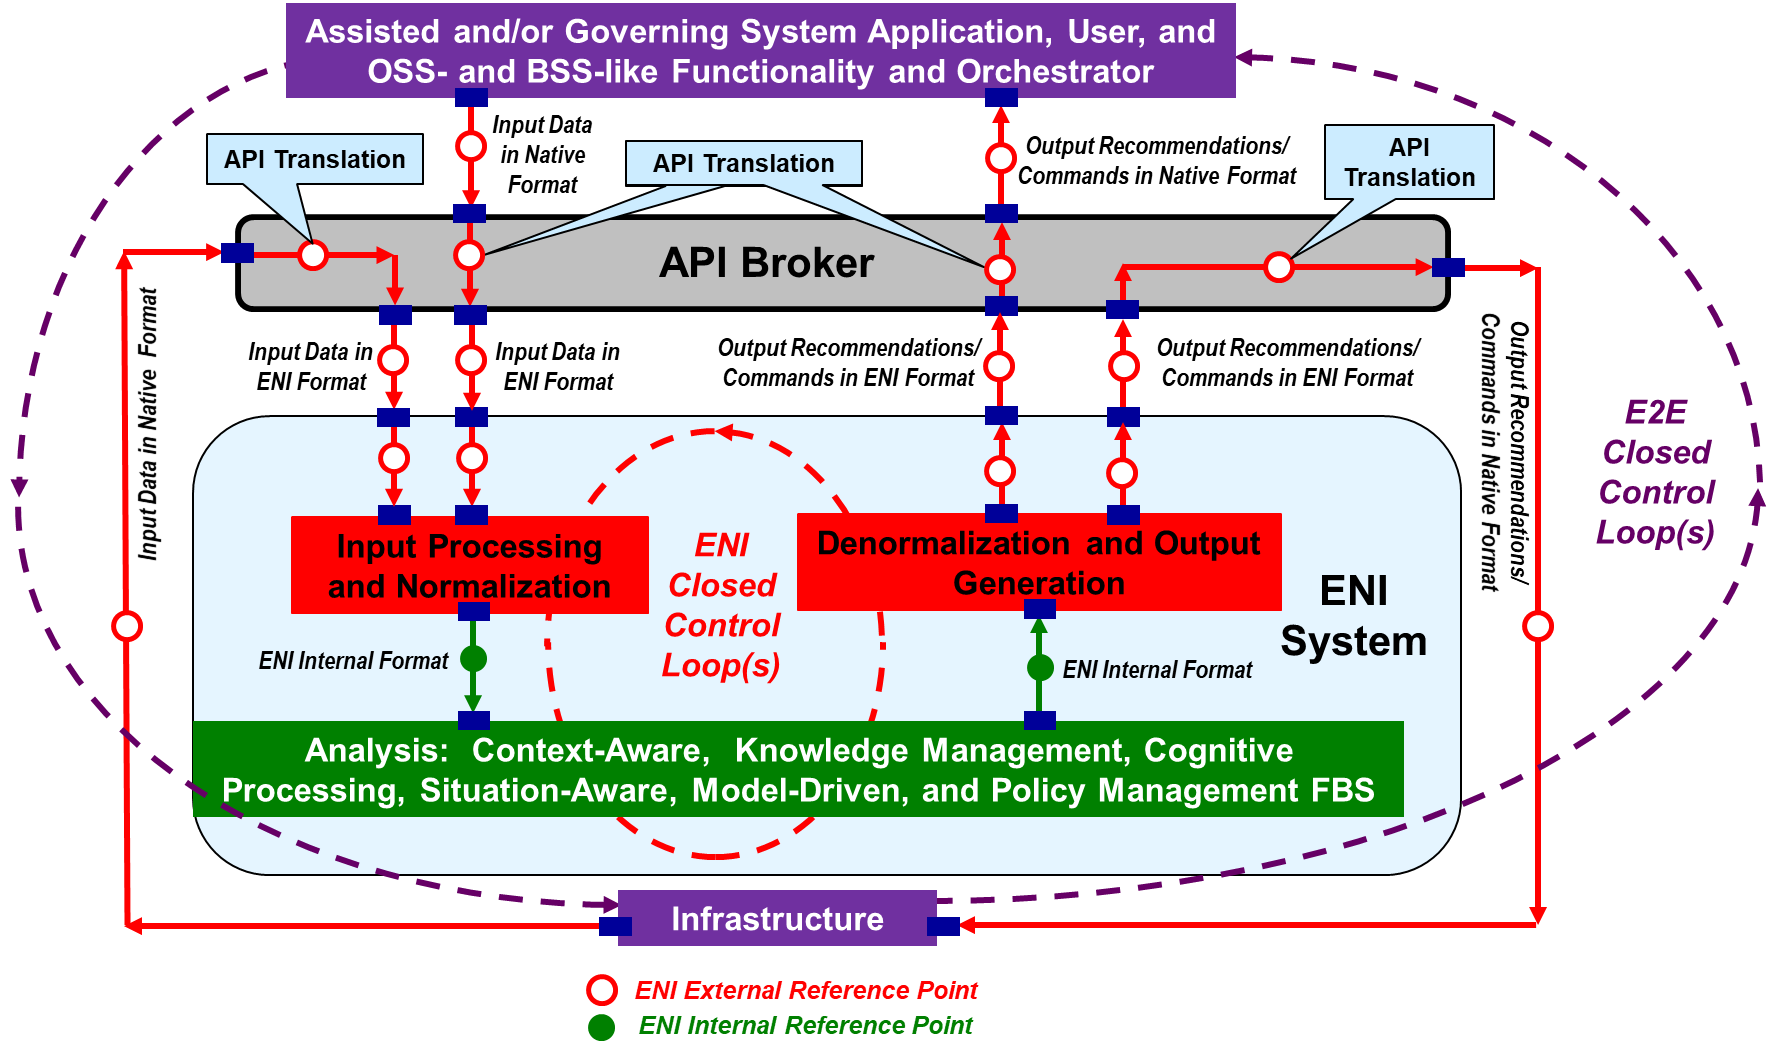
\includegraphics[width=1\linewidth]{23-eni-arch.png}
    \caption{Wysokopoziomowa architektura funkcjonalna ENI}\label{fig:23-eni-arch}
\end{figure}

Wysokopoziomową architekturę funkcjonalną ENI pokazano na rysunku \ref{fig:23-eni-arch}. Jej działanie można opisać jako dwie \textit{zamknięte pętle sterowania}. Za pomocą zewnętrznej, system zarządzania (użytkownik, OSS/BSS, orkiestrator) reguluje pracę sieci (infrastruktury). Dokonuje tego nie bezpośrednio, lecz za pomocą ENI System, który sam wewnętrznie również posiada zamkniętą pętle sterowania. Wewnętrzna pętla podczas wnioskowania bierze pod uwagę nie tylko wiedzę płynącą bezpośrednio z sieci, ale również tę od orkiestratora. Wszystkie komponenty odpowiedzialne za sztuczną inteligencję są umieszczone na rysunku \ref{fig:23-eni-arch} w zielonym prostokącie i stanowią \textit{workflow} wewnętrznej pętli. 